 Для следующих двух заданий будем использовать следующее изображение:

 \begin{figure}[ht!]
    \centering
    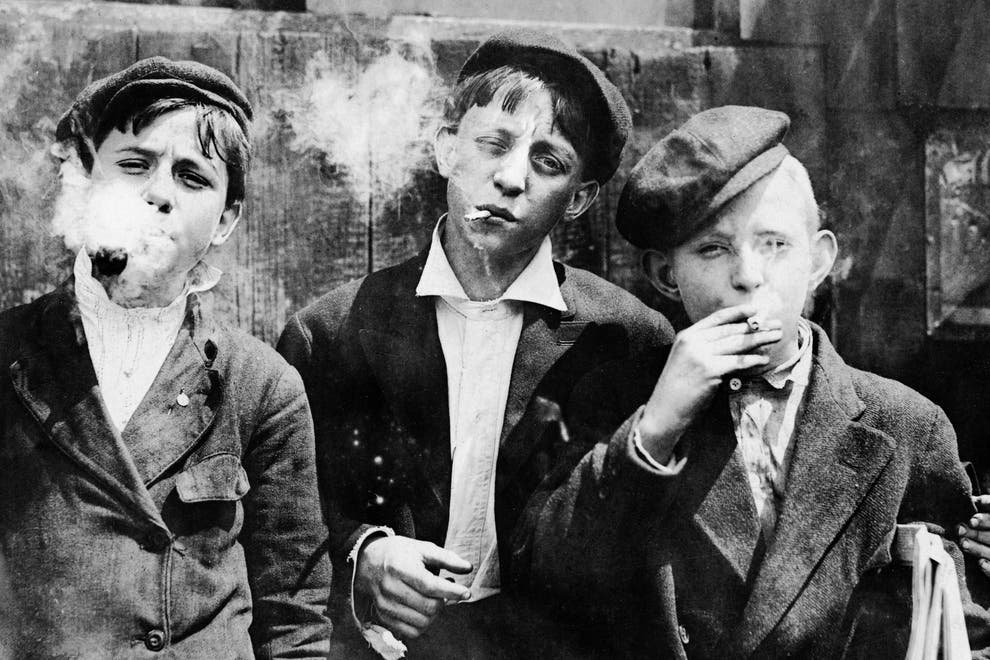
\includegraphics[width=0.95\textwidth]{images/source_images/task_2_3/smoking-boys.jpg}
    \caption{Lewis Hine -- 11:00 A.M. Monday, May 9th, 1910. Newsies at Skeeter's Branch, Jefferson near Franklin. They were all smoking. Location- St. Louis, Missouri}
    \label{fig:smoking_boys}
\end{figure}

 \subsection{Размытие изображения}
 \subsubsection{Блочное размытие}

 Для выполнения блочного размытия необходимо использовать квадратную матрицу $N \times N$, элементами которой являются дроби $\frac{1}{N}$. Рассмотрим и сравним блочное размытие при $N=5, 9, 11$ при помощи свертки и перемножения Фурье-образов с последующим обратным преобразованием.

 \begin{figure}[ht!]
    \centering
    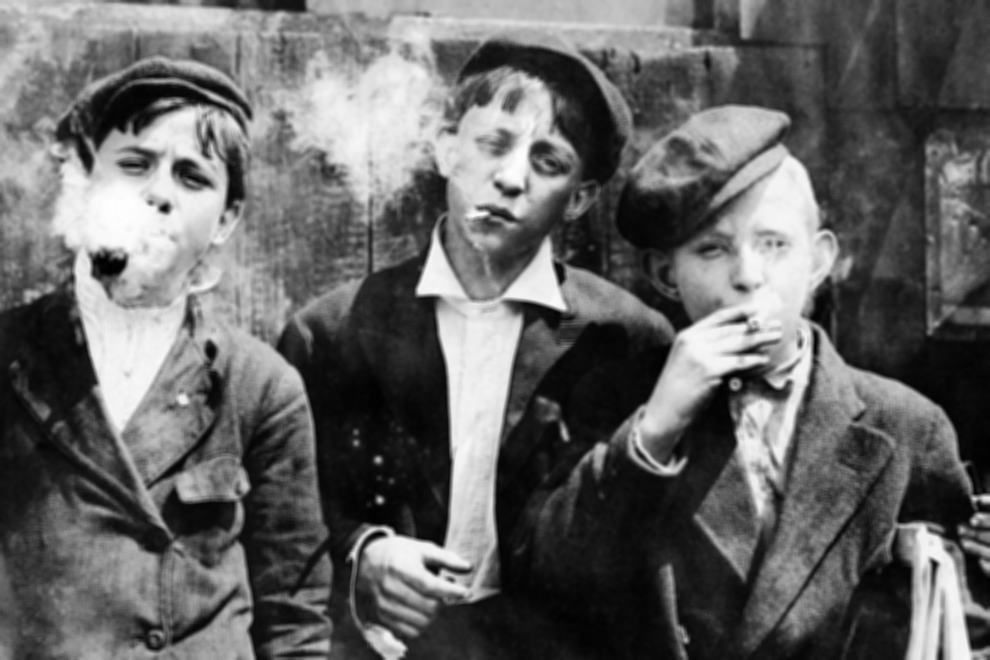
\includegraphics[width=0.95\textwidth]{images/result/task_2/Averaging_5.png}
    \caption{Результат блочного размытия при помощи свертки при $N=5$}
    \label{fig:av_c_5}
\end{figure}

\begin{figure}[ht!]
    \centering
    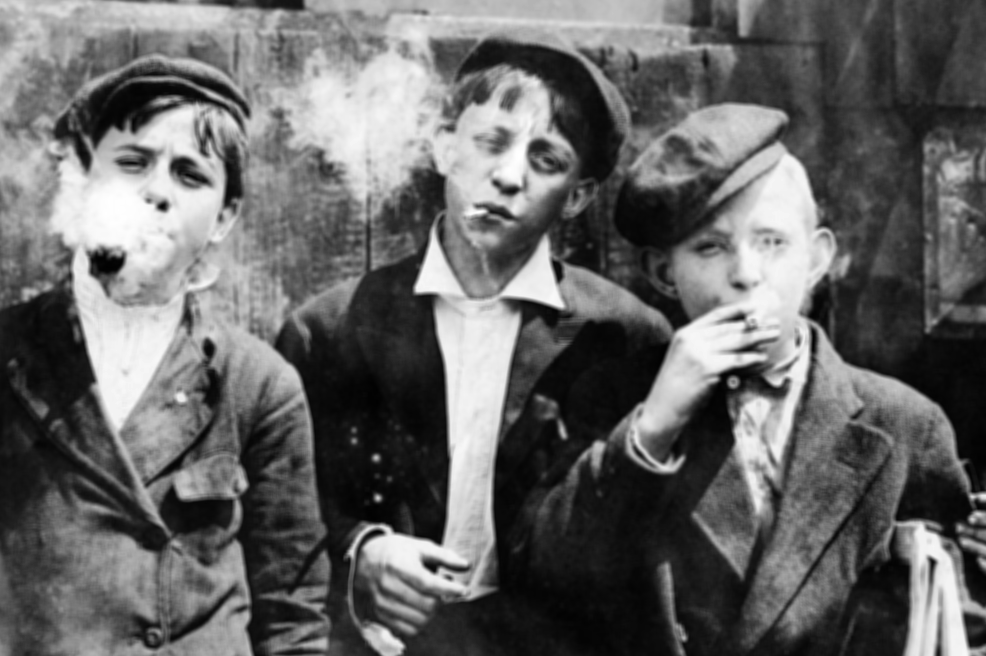
\includegraphics[width=0.95\textwidth]{images/result/task_2/Averaging_fourier_5.png}
    \caption{Результат блочного размытия при помощи преобразований Фурье при $N=5$}
    \label{fig:av_f_5}
\end{figure}

\begin{figure}[ht!]
    \centering
    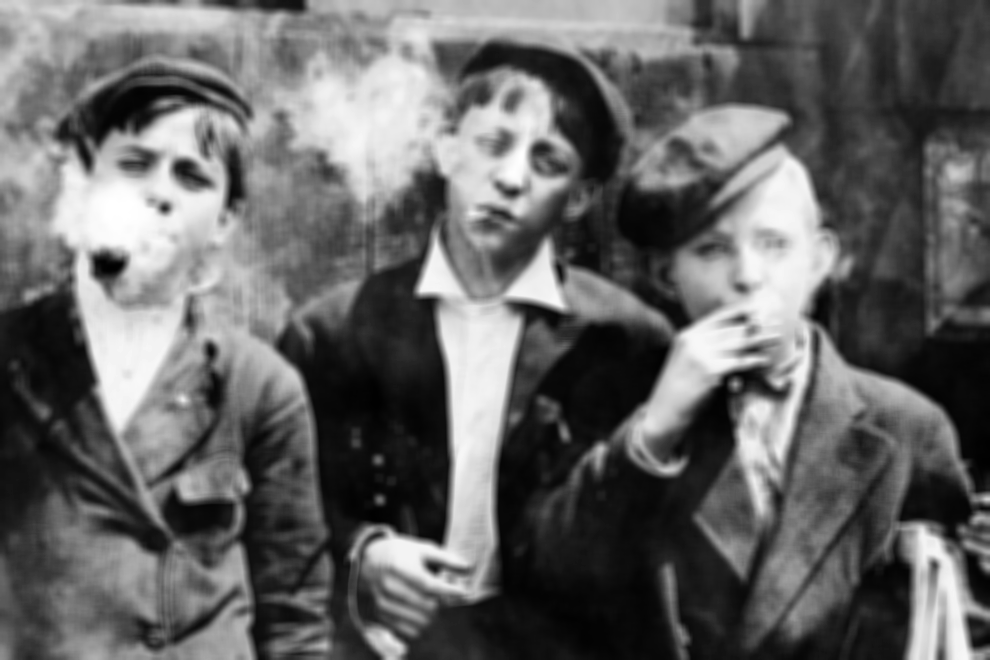
\includegraphics[width=0.95\textwidth]{images/result/task_2/Averaging_9.png}
    \caption{Результат блочного размытия при помощи свертки при $N=9$}
    \label{fig:av_c_9}
\end{figure}

\begin{figure}[ht!]
    \centering
    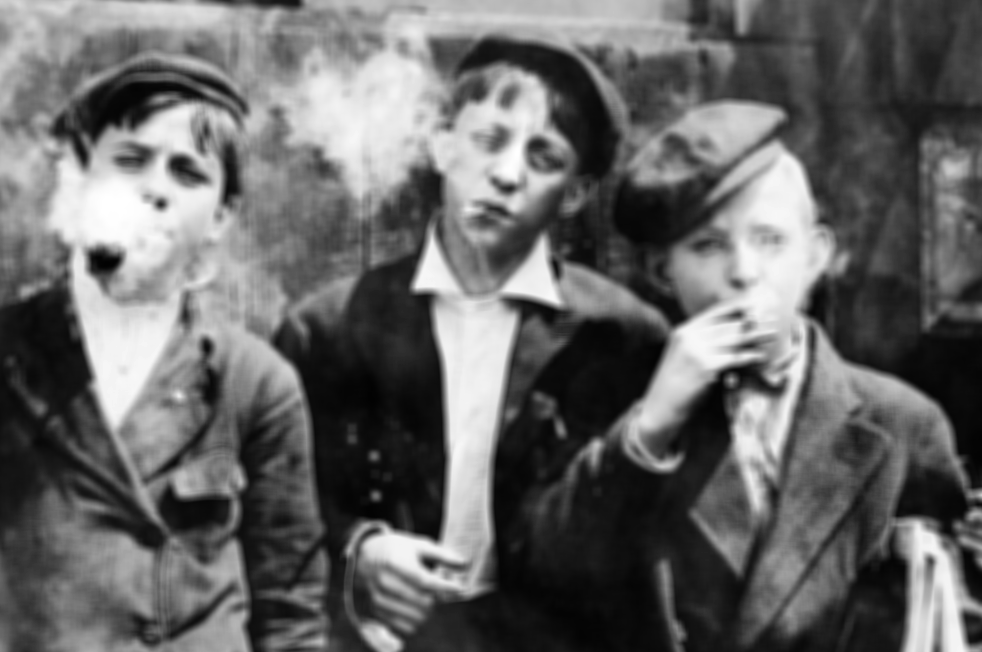
\includegraphics[width=0.95\textwidth]{images/result/task_2/Averaging_fourier_9.png}
    \caption{Результат блочного размытия при помощи преобразований Фурье при $N=9$}
    \label{fig:av_f_9}
\end{figure}

\begin{figure}[ht!]
    \centering
    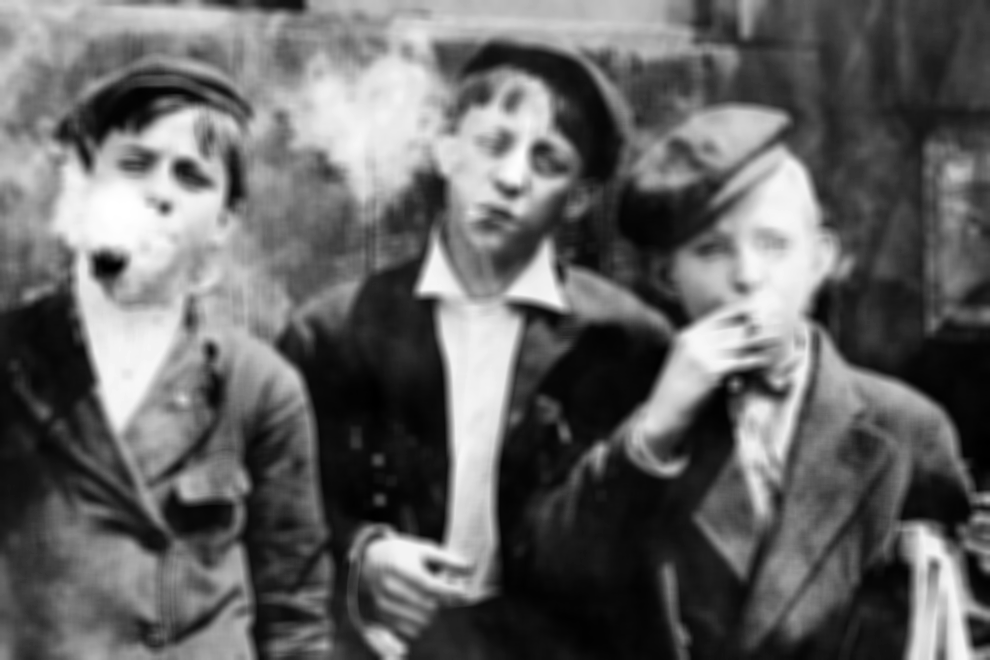
\includegraphics[width=0.95\textwidth]{images/result/task_2/Averaging_11.png}
    \caption{Результат блочного размытия при помощи свертки при $N=11$}
    \label{fig:av_c_11}
\end{figure}

\begin{figure}[ht!]
    \centering
    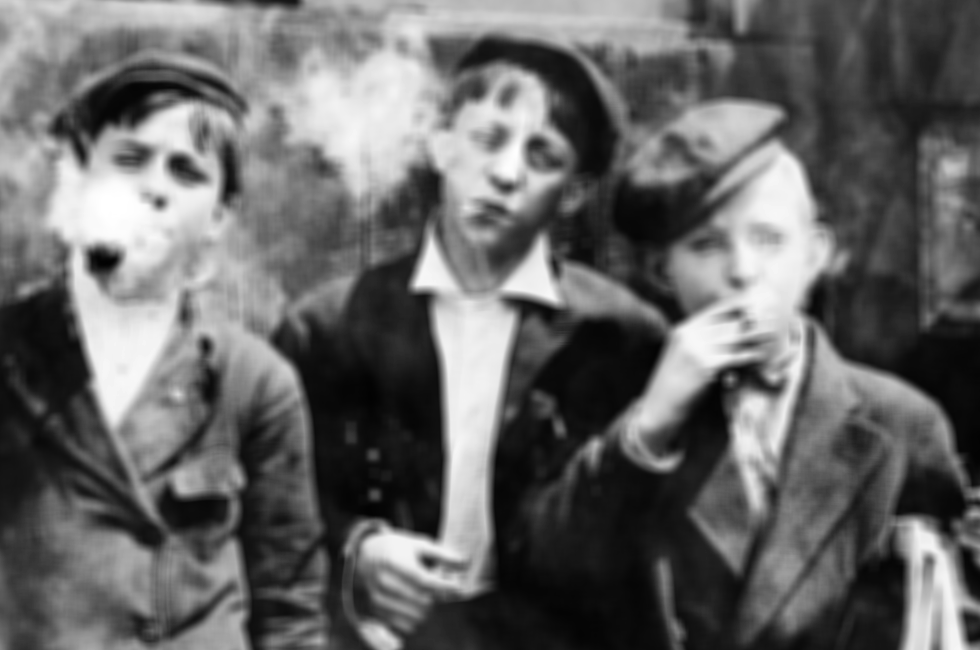
\includegraphics[width=0.95\textwidth]{images/result/task_2/Averaging_fourier_11.png}
    \caption{Результат блосного размытия при помощи преобразований Фурье при $N=11$}
    \label{fig:av_f_11}
\end{figure}
Полученные результаты идентичны, что подтверждает эквивалентность свертки и произведения Фурье-образов.
\clearpage
\subsubsection{Гауссово размытие}

Переходим к размытию по Гауссу при $N=5, 9, 11$:
\begin{figure}[ht!]
    \centering
    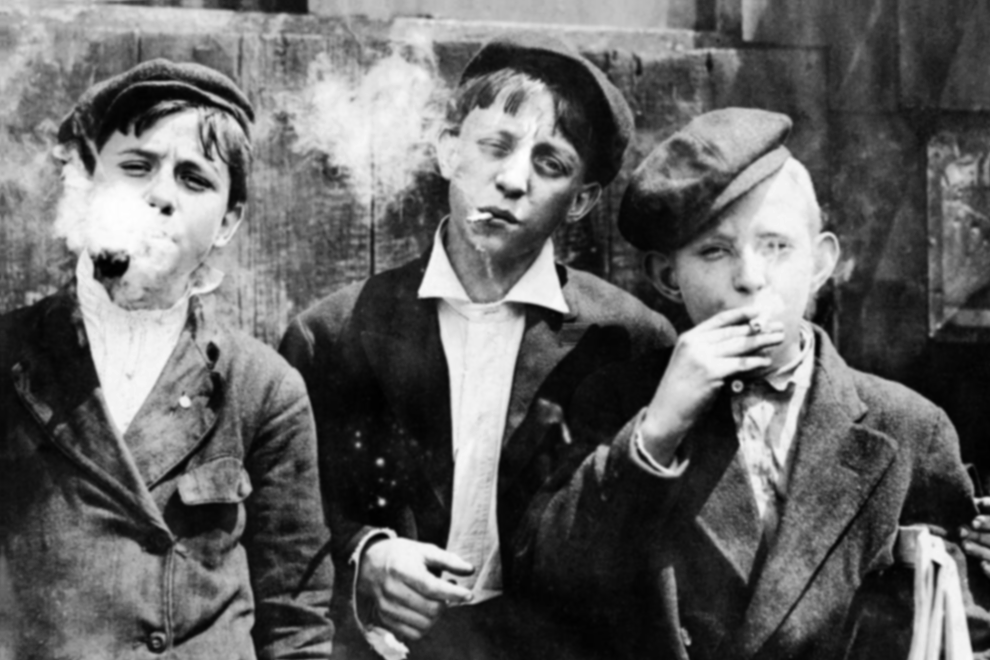
\includegraphics[width=0.85\textwidth]{images/result/task_2/Gaussian_5.png}
    \caption{Результат размытия по Гауссу при помощи свертки при $N=5$}
    \label{fig:ga_c_5}
\end{figure}

\begin{figure}[ht!]
    \centering
    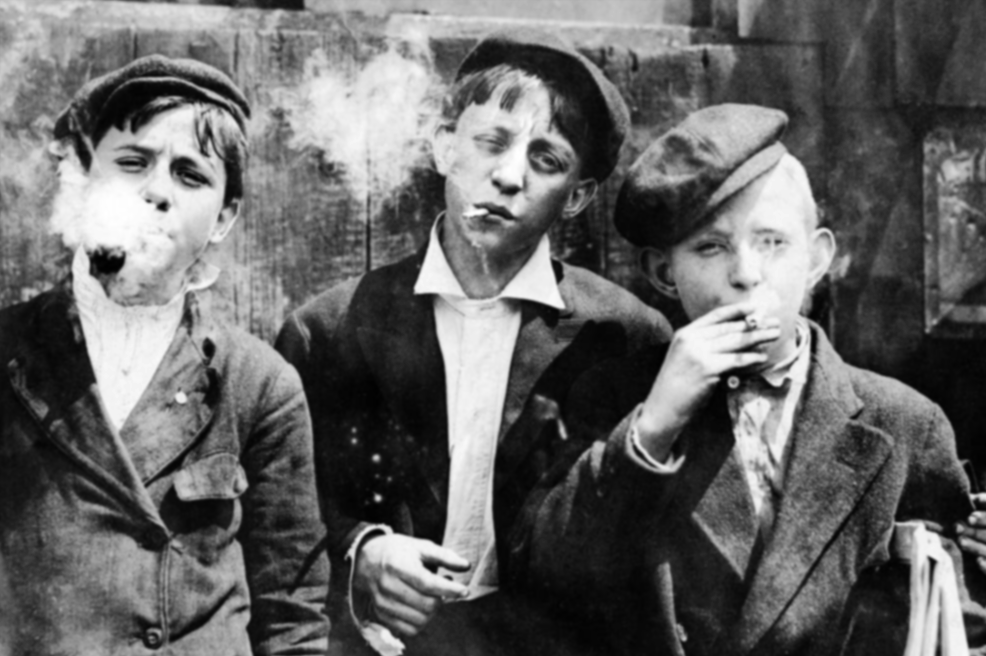
\includegraphics[width=0.85\textwidth]{images/result/task_2/Gaussian_fourier_5.png}
    \caption{Результат размытия по Гауссу при помощи преобразований Фурье при $N=5$}
    \label{fig:ga_f_5}
\end{figure}

\begin{figure}[ht!]
    \centering
    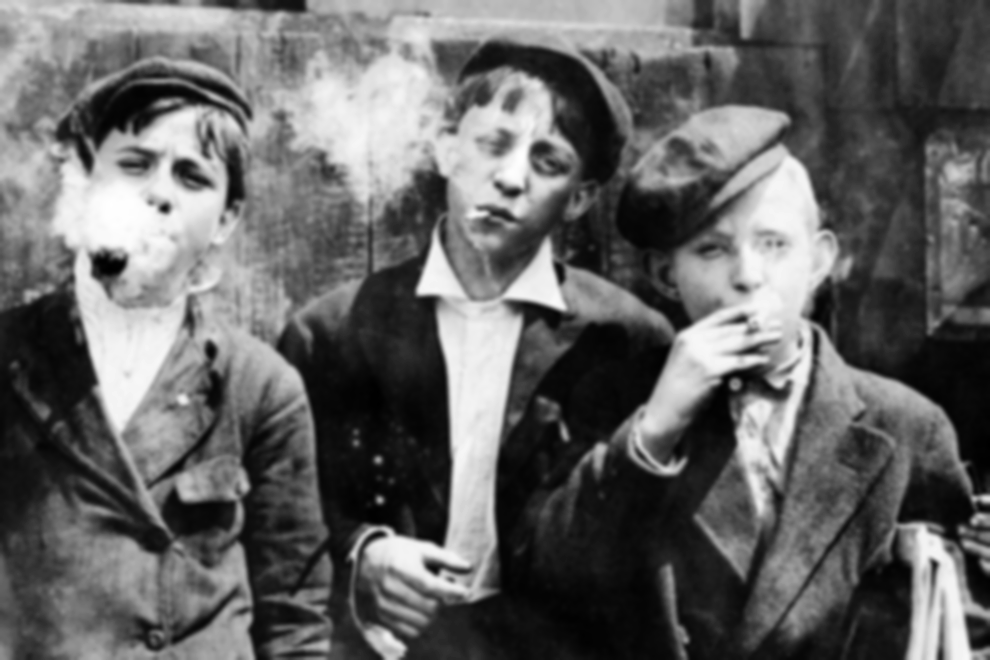
\includegraphics[width=0.95\textwidth]{images/result/task_2/Gaussian_9.png}
    \caption{Результат размытия по Гауссу при помощи свертки при $N=9$}
    \label{fig:ga_c_9}
\end{figure}

\begin{figure}[ht!]
    \centering
    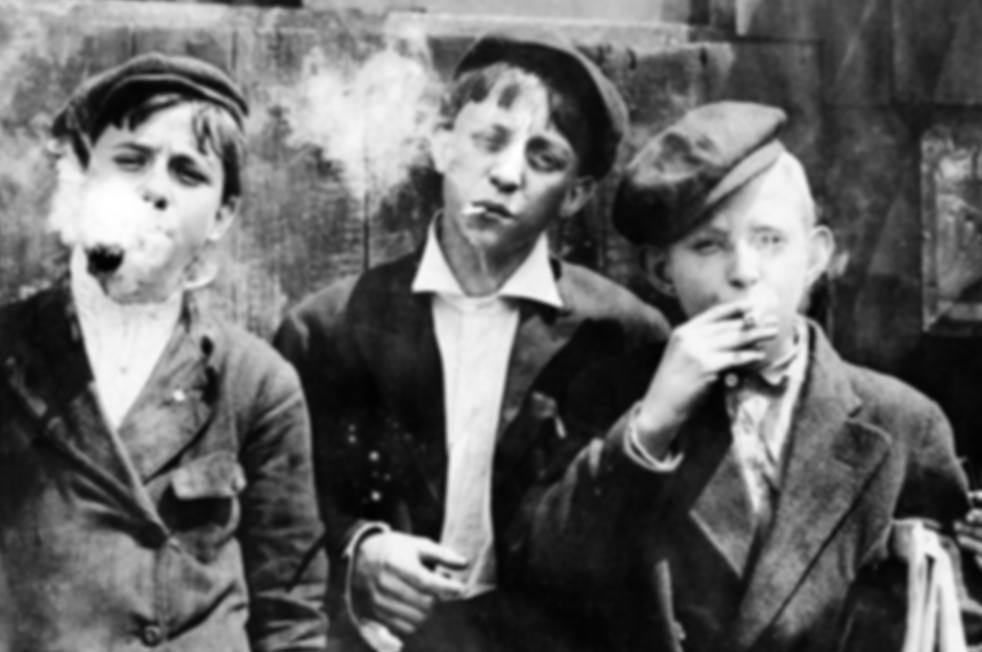
\includegraphics[width=0.95\textwidth]{images/result/task_2/Gaussian_fourier_9.png}
    \caption{Результат размытия по Гауссу при помощи преобразований Фурье при $N=9$}
    \label{fig:ga_f_9}
\end{figure}

\begin{figure}[ht!]
    \centering
    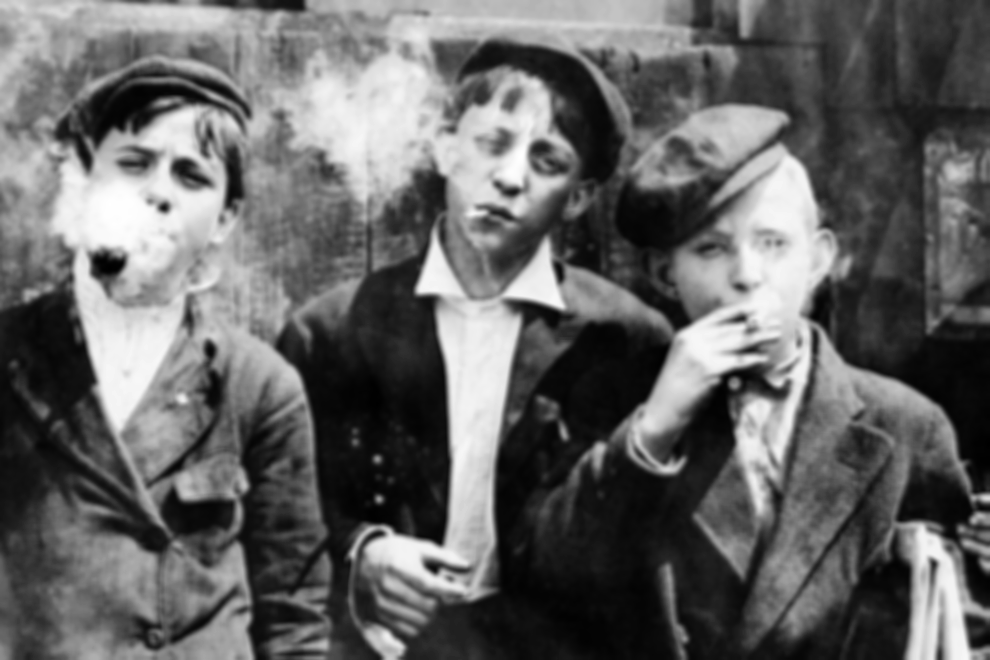
\includegraphics[width=0.95\textwidth]{images/result/task_2/Gaussian_11.png}
    \caption{Результат размытия по Гауссу при помощи свертки при $N=11$}
    \label{fig:ga_c_11}
\end{figure}

\begin{figure}[ht!]
    \centering
    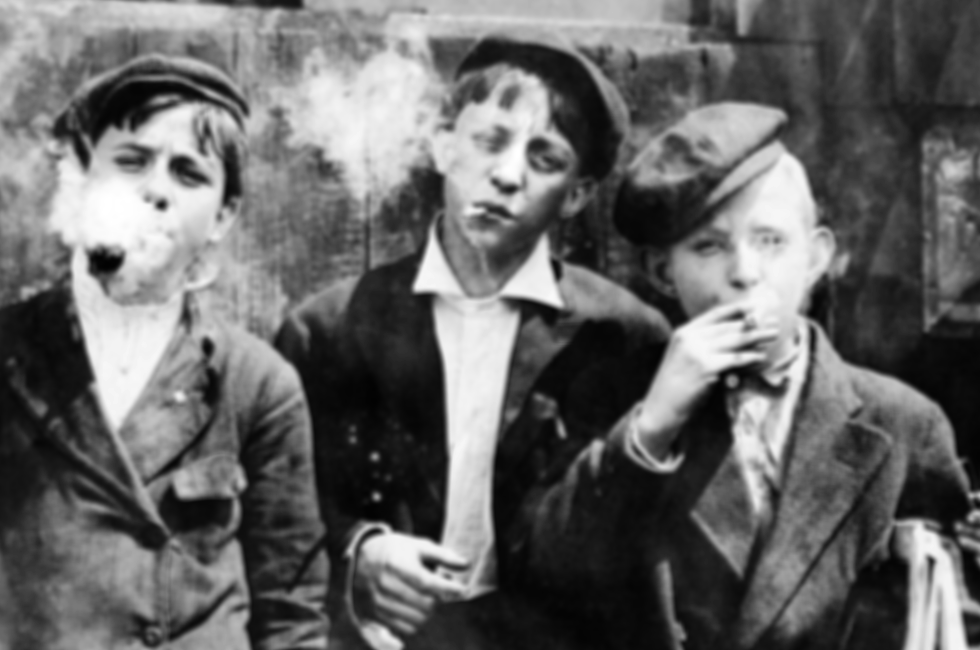
\includegraphics[width=0.95\textwidth]{images/result/task_2/Gaussian_fourier_11.png}
    \caption{Результат размытия по Гауссу при помощи преобразований Фурье при $N=11$}
    \label{fig:ga_f_11}
\end{figure}

Мы снова получили идентичные друг другу изображения. 

Результат гауссовского размытия получается более сглаженным в сравнении с блочным, будто на изображении лежит полупрозрачное стекло. Во втором случае возникает ощущение, что результат -- <<смазанное>> изображение более низкого качетсва.

